\documentclass[conference]{IEEEtran}
\IEEEoverridecommandlockouts
% The preceding line is only needed to identify funding in the first footnote. If that is unneeded, please comment it out.
\usepackage{cite}
\usepackage{amsmath,amssymb,amsfonts}
\usepackage{algorithmic}
\usepackage{graphicx}
\usepackage{textcomp}
\usepackage{xcolor}
\usepackage{hyperref}

\def\BibTeX{{\rm B\kern-.05em{\sc i\kern-.025em b}\kern-.08em
    T\kern-.1667em\lower.7ex\hbox{E}\kern-.125emX}}

\graphicspath{{../outputs/plots/}{plots/}}

\begin{document}

\title{Robust Medical Vision: Designing Uncertainty-Aware Classifiers for Pulmonary Diagnosis}

\author{\IEEEauthorblockN{1\textsuperscript{st} Prince Sahoo}
\IEEEauthorblockA{\textit{School of Computer Science} \\
\textit{Academic Projects}\\
princesahoo@example.com}
}

\maketitle

\begin{abstract}
Clinical artificial intelligence systems must know when they do not know. 
This report details the foundational methodology for an AI product designed to diagnose chest X-rays (NORMAL vs. PNEUMONIA) safely. 
We establish a robust pipeline from exploratory data analysis to feature engineering using Histograms of Oriented Gradients (HOG) and Local Binary Patterns (LBP). 
By training classical vision classifiers under an uncertainty-aware framework, our project aims to handle anomalous inputs, rare conditions, and out-of-distribution (OOD) cases to prevent confident yet incorrect medical predictions.
\end{abstract}

\begin{IEEEkeywords}
Uncertainty-Aware Modeling, Confidence Calibration, Medical AI, Chest X-Rays, Feature Engineering.
\end{IEEEkeywords}

\section{Introduction}
Modern clinical AI systems demonstrate remarkable diagnostic performance. 
However, their adoption is heavily hindered by \textit{uncertainty} and \textit{overconfidence}. 
A critical requirement for clinical safety is that AI models must explicitly understand and broadcast their lack of knowledge when encountering out-of-distribution (OOD) samples or inherently ambiguous diagnoses \cite{begoli2019need}.

The objective of this project is to mirror how state-of-the-art medical AI pipelines build safety mechanisms against unsafe predictions. 
Specifically, we address a binary classification task applied to the Kaggle Chest X-Ray Pneumonia dataset. 
While a naive "black-box" neural network might confidently predict either normal or pneumonia for an unexpected scan, we propose learning \textit{uncertainty-aware modeling} techniques \cite{kompa2021second}. 
Our methodology encompasses rigorous data pre-processing, engineered classical vision representation, and baseline machine learning evaluations designed to later compare confidence calibration strategies.

\section{Exploratory Data Analysis}
A meticulous Exploratory Data Analysis (EDA) of the raw lung radiographs dictates the downstream pipeline. Several critical findings forced our modeling decisions:
\begin{itemize}
    \item \textbf{Class Imbalance:} The training split manifests a 3:1 ratio of pneumonia to normal cases. This class skew necessitates using the Area Under the Receiver Operating Characteristic Curve (AUC-ROC) rather than raw accuracy.
    \item \textbf{Visual Texture \& Brightness:} \textit{Pneumonia} scans reveal hazy, broad white consolidation patches \cite{kermany2018identifying}. Statistically, pneumonia images yield measurably higher global brightness across the [0, 255] spectrum.
    \item \textbf{Spatial Localization:} Pathology tends to concentrate in the lower to middle lung zones, proven via spatial intensity heatmaps created across $3\times3$ lung grid patches.
    \item \textbf{Scanner Variations:} Image sizes display massive variation across different clinical scanners. This necessitates strict physical resizing and hints at structural OOD threats.
\end{itemize}

\begin{figure}[htbp]
    \centering
    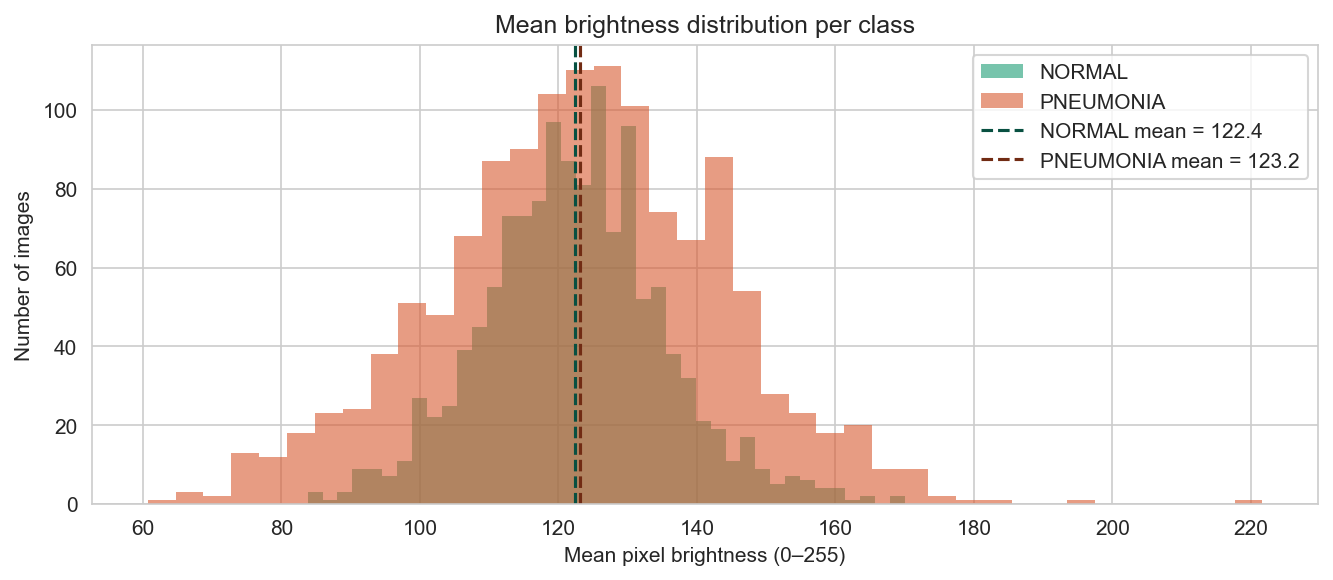
\includegraphics[width=\columnwidth]{eda_brightness_distribution.png}
    \caption{Mean brightness histogram showcasing the inherent intensity discrepancy between NORMAL and PNEUMONIA scans.}
    \label{fig:brightness}
\end{figure}

\section{Methodology}

\subsection{Preprocessing Pipeline}
Given the varied raw output of hospital scanners (Finding 5), a strict normalization process is required prior to any feature extraction. As X-rays carry structurally defining signals in luminosity rather than chroma, the images are loaded exclusively in grayscale matrices. They are then resized to a static $128 \times 128$ pixel spatial frame to allow uniform feature dimensionalities. 
Finally, pixel bounds are min-max scaled to $[0.0, 1.0]$. Training arrays are uniformly shuffled to unseat temporal class-sorting biases \cite{kermany2018identifying}. 

\subsection{Feature Engineering}
Based directly on the textural and edge-heavy observations of the dataset, two complimentary mathematical representation metrics are extracted to summarize structural and semantic features in a lower-dimensional topology:
\begin{enumerate}
    \item \textbf{Histograms of Oriented Gradients (HOG):} HOG maps structural gradient geometry \cite{dalal2005histograms}. In pneumonic lung cases, abnormal internal borders formed by fluid consolidations emerge as pronounced, multi-directional edge vectors that break the uniformity of healthy rib-cages space.
    \item \textbf{Local Binary Patterns (LBP):} Acting iteratively on pixel-neighborhoods, LBP describes micro-textural patterns \cite{ojala2002multiresolution}. Normal lung spaces maintain highly uniform LBP codes, while the clouded presence of infections yields noisy, irregular neighborhood patterns visible tightly across the histogram bins.
\end{enumerate}

These spatial metrics form a combined feature array comprising roughly 1,144 descriptors, compressing $16,384$ pixels into dense semantic signals highly receptive to classical margin classifiers.

\begin{figure}[htbp]
    \centering
    \includegraphics[width=\columnwidth]{feature_hog_visualization.png}
    \caption{HOG edge gradients visibly isolating pneumonic fluid boundaries from structurally uniform healthy rib-spaces.}
    \label{fig:hog}
\end{figure}

\section{Advanced Modeling and Uncertainty Calibration}
With engineered structural tokens, we implement non-deep modeling algorithms—specifically Support Vector Machines (SVM), Logistic Regressions, and K-Nearest Neighbors (KNN)—as our Baseline ML approach. The focus will strictly remain on interpreting decision boundary distances, probability calibration via techniques like Platt Scaling or Isotonic Regression, and mapping out-of-distribution (OOD) rejection thresholds \cite{guo2017calibration}. 

By steering away from inherently uncalibrated, over-parametrized deep neural networks for the baseline, we force the AI to return soft-probabilities directly tied to geometric distances within our engineered $1144$-D feature space.

\section{Conclusion and Scope for Future Work}
Reliable clinical AI cannot be a monolithic "black box". By standardizing medical radiographs and breaking them into classical texture properties, we lay the groundwork for intrinsically interpretative medical classifiers. Future efforts on this pipeline will evaluate differing confidence calibration techniques aiming to safely halt false-positive assessments, bridging the gap from simple prediction to uncertainty-aware diagnosis.

\section*{Acknowledgment}

We acknowledge the public availability of the primary Kaggle Chest X-Ray Pneumonia datasets that powered the evaluation structure of this work.

\bibliographystyle{IEEEtran}
\bibliography{references}

\end{document}
